\documentclass[11pt]{article}

\usepackage{amsmath,amssymb}
\usepackage{geometry}
\usepackage{hyperref}
\usepackage{graphicx}
\usepackage{booktabs}
\usepackage{enumitem}
\usepackage{float}
\geometry{margin=1in}

\title{Optimization Log Copilot: Using Large Language Models to Analyze Mathematical Optimization Solver Logs}
\author{Jeff Ginn \\ EN.705.605 Introduction to Generative AI}
\date{\today}

\begin{document}
\maketitle

% ============================================================
\begin{abstract}
Modern optimization solvers for linear programming (LP) and mixed-integer programming (MIP) produce detailed logs describing solver progress, including presolve reductions, 
cutting plane generation, branching decisions, heuristic activity, and bound progression. Interpreting these logs to diagnose performance bottlenecks requires significant 
domain expertise and manual effort, limiting accessibility for many practitioners. This paper presents the Optimization Log Copilot, a system that leverages large language models (LLMs) 
to automatically analyze solver logs and generate structured diagnostic summaries. The proposed approach combines structured log parsing with transformer-based sequence understanding 
and generative language models to perform three tasks: log summarization, performance issue detection, and solver recommendation generation. We describe the system architecture, 
a dataset of approximately 200 solver logs collected from MIPLIB 2017 benchmarks and Ramsey-type problems from the Rose solver, and a multi-label classification framework for bottleneck detection. 
Preliminary results from prototype development demonstrate the feasibility of structured log parsing and rule-based diagnostic generation, with planned experiments to evaluate LLM-based 
approaches using metrics including precision, recall, F1 score, ROUGE, and human expert evaluation.
\end{abstract}

% ============================================================
\section{Introduction}
\label{sec:intro}

Modern optimization solvers for linear programming (LP) and mixed-integer linear programming (MILP) produce logs that describe solver progress in detail, including presolve activity, 
cut generation, heuristic behavior, branching decisions, node exploration, optimality gap progression, and termination status. While these logs contain valuable diagnostic 
information, they are difficult to interpret without deep expertise in optimization algorithms. As a result, users often struggle to understand why a solver run is slow, 
fails to converge, or exhibits unstable behavior. Diagnosing these issues typically requires manual inspection, which limits accessibility and productivity.

The difficulty of solver log analysis stems from several factors. First, solver logs are semi-structured text that mix numerical output with free-form status messages. 
Second, the logs can be extremely long, sometimes containing thousands of lines for a single solve. Third, the terminology and metrics are domain-specific: concepts 
such as LP relaxation gaps, simplex pivots, Gomory cuts, and branching pseudocosts require familiarity with mathematical optimization theory. Finally, the patterns 
that indicate performance issues are often subtle and context-dependent. For example, a large root LP gap alone may or may not indicate a weak formulation, depending 
on the problem structure and subsequent bound improvement.

Recent advances in large language models (LLMs) have demonstrated strong capabilities in processing semi-structured text, including system log analysis for 
incident detection \cite{akhtar2025llmbasedeventloganalysis}, anomaly detection in software infrastructure \cite{landauer2023deeplearningloganomaly}, and reasoning 
over structured data. However, these techniques have been applied primarily to IT system logs and software engineering contexts, not to mathematical optimization solver logs.

This project explores whether LLMs can serve as an ``Optimization Log Copilot'' that automatically analyzes solver logs and provides diagnostic insights about solver performance. 
The system aims to answer questions such as: Why is the solver exploring a large number of nodes? Is the root LP relaxation weak? Are cutting planes improving the bound? 
What structural issues might exist in the optimization model?

The proposed approach combines structured log parsing with transformer-based sequence understanding and conditional text generation. The system is designed as a 
post-processing advisory layer that operates independently of solver internals. The ML problems addressed include multi-label classification for bottleneck detection and 
sequence-to-sequence generation for diagnostic explanation.

The remainder of this paper is organized as follows. 
Section~\ref{sec:related_work} surveys related work in LLM-based log analysis, deep learning for anomaly detection, 
and machine learning for combinatorial optimization. 
Section~\ref{sec:problem} defines the research problem and hypotheses. 
Section~\ref{sec:method} describes the proposed method, including the system architecture, dataset, and training approach. 
Section~\ref{sec:experiments} outlines the planned experimental evaluation. 
Section~\ref{sec:results} presents results. 
Section~\ref{sec:conclusion} discusses conclusions and future directions.


% ============================================================
\section{Related Work}
\label{sec:related_work}

Several research areas inform this project: LLM-based log analysis, deep learning for anomaly detection in log data, and machine learning for combinatorial optimization.

\subsection{LLM-Based Log Analysis}

Akhtar et al.\ \cite{akhtar2025llmbasedeventloganalysis} survey how large language models are being applied to event log analysis, particularly in system reliability and 
software engineering contexts. They identify that traditional approaches to log analysis require heavy feature engineering, depend on rigid log parsing, and struggle with 
unstructured or evolving log formats. The survey categorizes LLM-based approaches into four groups: fine-tuning, in-context learning, retrieval-augmented generation (RAG), 
and hybrid symbolic--LLM systems. A key finding is that RAG is strongly preferred over fine-tuning for log analysis because fine-tuning LLMs on logs is expensive and brittle, 
while RAG performs well with smaller datasets and reduces hallucination risk. The survey also notes that log analysis evaluation often lacks ground truth and that human judgment 
remains necessary, suggesting that an LLM-based copilot should supplement rather than replace human reasoning.

\subsection{Deep Learning for Anomaly Detection in Log Data}

Landauer et al.\ \cite{landauer2023deeplearningloganomaly} survey deep learning methods for log anomaly detection, covering system failures, incidents, intrusions, and operational 
breakdowns. The methods reviewed include sequence-based models (LSTMs, GRUs, and Transformer architectures), reconstruction-based models (autoencoders and variational autoencoders), 
and graph-based methods. Key findings include that transformer models outperform LSTMs in modeling long-range dependencies, and that deep models generally outperform classical 
statistical anomaly detectors, with reported F1 scores ranging from 0.90 to 0.98 for deep LSTM-based models and often exceeding 0.95 for transformer-based approaches. Common 
evaluation metrics include precision, recall, F1 score, and ROC-AUC. However, these systems have been applied primarily to software infrastructure logs rather than optimization solver logs, 
leaving the domain of solver diagnostics largely unexplored.

\subsection{Machine Learning for Combinatorial Optimization}

Bengio et al.\ \cite{bengio2018mlforcombinatorial} survey how machine learning can assist combinatorial optimization solvers by learning decision policies. They categorize ML usage 
into learning to configure (parameter tuning, solver selection), learning to guide search (branching policies, cut selection, node selection), learning surrogate models (predicting 
solver runtime and node counts), and reinforcement learning for search policies. The survey reports that learned branching strategies can yield 10--30\% runtime reductions over 
handcrafted heuristics, and that ML-based solver configuration can reduce runtime significantly. For this project, the survey underscores that ML-driven solver diagnostics and decision 
support are important research directions, particularly for recommending parameter settings such as cut aggressiveness, heuristic configurations, and presolve adjustments based on log analysis.

Kotary et al.\ \cite{kotary2021endtoend} survey end-to-end constrained optimization learning, providing additional context on how ML models can be integrated with optimization solvers. 
Yazdani et al.\ \cite{yazdani2025evocut} demonstrate how language models can be used to strengthen integer programs through evolution-guided cut generation, illustrating a direct connection 
between LLMs and optimization solver improvement.

\subsection{Gap in the Literature}

While LLM-based log analysis has been studied extensively for IT infrastructure and software systems, and machine learning has been applied to various aspects of optimization solver control, 
using LLMs to analyze and diagnose optimization solver logs remains largely unexplored. Optimization researchers typically analyze solver logs manually through ad hoc inspection of 
branch-and-bound traces, cut effectiveness metrics, and solver benchmarking output. Automated interpretation tools for solver logs are rare. This project addresses that gap.

% ============================================================
\section{Research Problem and Hypotheses}
\label{sec:problem}

\subsection{Problem Description}

Solver logs are semi-structured sequences containing solver events, numerical metrics, and domain-specific terminology. Modern solvers internally adapt their behavior based on problem structure 
adjusting branching strategies, selecting cuts, and configuring heuristics, but this information is encoded in log output that is not easily accessible to users. 
The research problem addressed in this project is:

\begin{quote}
\emph{Given a raw solver log from a LP/MIP solver, can a machine learning system generate a structured diagnostic summary and identify likely performance bottlenecks?}
\end{quote}

Typical performance issues that the system should detect include:

\begin{itemize}
    \item Weak LP relaxation: Large initial optimality gap at the root node, indicating the LP relaxation provides a poor bound.
    \item Excessive branching: Exploding node counts during branch-and-bound search, often caused by weak variable selection or symmetry.
    \item Ineffective cut generation: Many cutting plane rounds with little bound improvement.
    \item Degeneracy: Slow LP pivots and numerical instability during the simplex method.
    \item Insufficient presolve: Minimal problem reduction during the presolve phase.
\end{itemize}

\subsection{Primary Hypothesis}

The central claim of this project is:

\begin{quote}
\emph{A system that combines structured log parsing with large language model reasoning can analyze optimization solver logs and produce diagnostic outputs---bottleneck classifications, natural-language summaries, and solver recommendations---whose quality meets or exceeds that of rule-based baselines across all three tasks, as measured by F1 score, ROUGE, and expert evaluation.}
\end{quote}

This hypothesis is falsifiable: if the LLM-based approaches fail to outperform the rule-based heuristic baseline on any of the three metrics defined below, the hypothesis does not hold for that task. The hypothesis is decomposed into three sub-hypotheses, each tied to a specific performance metric.

\subsection{Sub-Hypotheses}

\begin{itemize}
    \item H1 (Bottleneck Detection): A transformer-based classifier operating on parsed solver log features can achieve a macro-averaged F1 score of at least 0.85 for multi-label bottleneck classification, matching the lower bound of F1 scores reported for deep learning log anomaly detectors in Landauer et al.\ \cite{landauer2023deeplearningloganomaly} (0.90--0.98 for LSTM models, $>$0.95 for transformer models). The 0.85 threshold accounts for the smaller dataset and more specialized domain.
    \item H2 (Summarization): An LLM-based system can generate natural-language summaries of solver log behavior that achieve ROUGE-L scores of at least 0.40 when compared to expert-written reference summaries. This threshold is grounded in ROUGE-L scores reported for abstractive summarization of technical documents, where scores in the 0.35--0.45 range indicate substantive alignment with reference text \cite{raffel2020t5}. Because solver log summaries require domain-specific terminology and precise numerical claims, exceeding 0.40 would demonstrate meaningful content overlap beyond generic language.
    \item H3 (Recommendation Quality): The system can produce solver configuration recommendations that domain experts rate as ``actionable and correct'' on at least 70\% of test cases, using a binary expert judgment protocol. This threshold is motivated by the finding in Akhtar et al.\ \cite{akhtar2025llmbasedeventloganalysis} that human judgment remains necessary for log analysis evaluation, and that LLM-based systems should supplement rather than replace expert reasoning. A 70\% actionability rate would demonstrate practical utility without requiring the system to match expert performance on every instance.
\end{itemize}

% ============================================================
\section{Method}
\label{sec:method}

The Optimization Log Copilot combines structured log parsing, transformer-based sequence understanding, and generative language models to produce both structured predictions and 
natural-language explanations. The system does not modify solver internals.

\subsection{System Architecture}

The system pipeline consists of four stages, shown in Figure~\ref{fig:architecture}.

\begin{figure}[H]
\centering
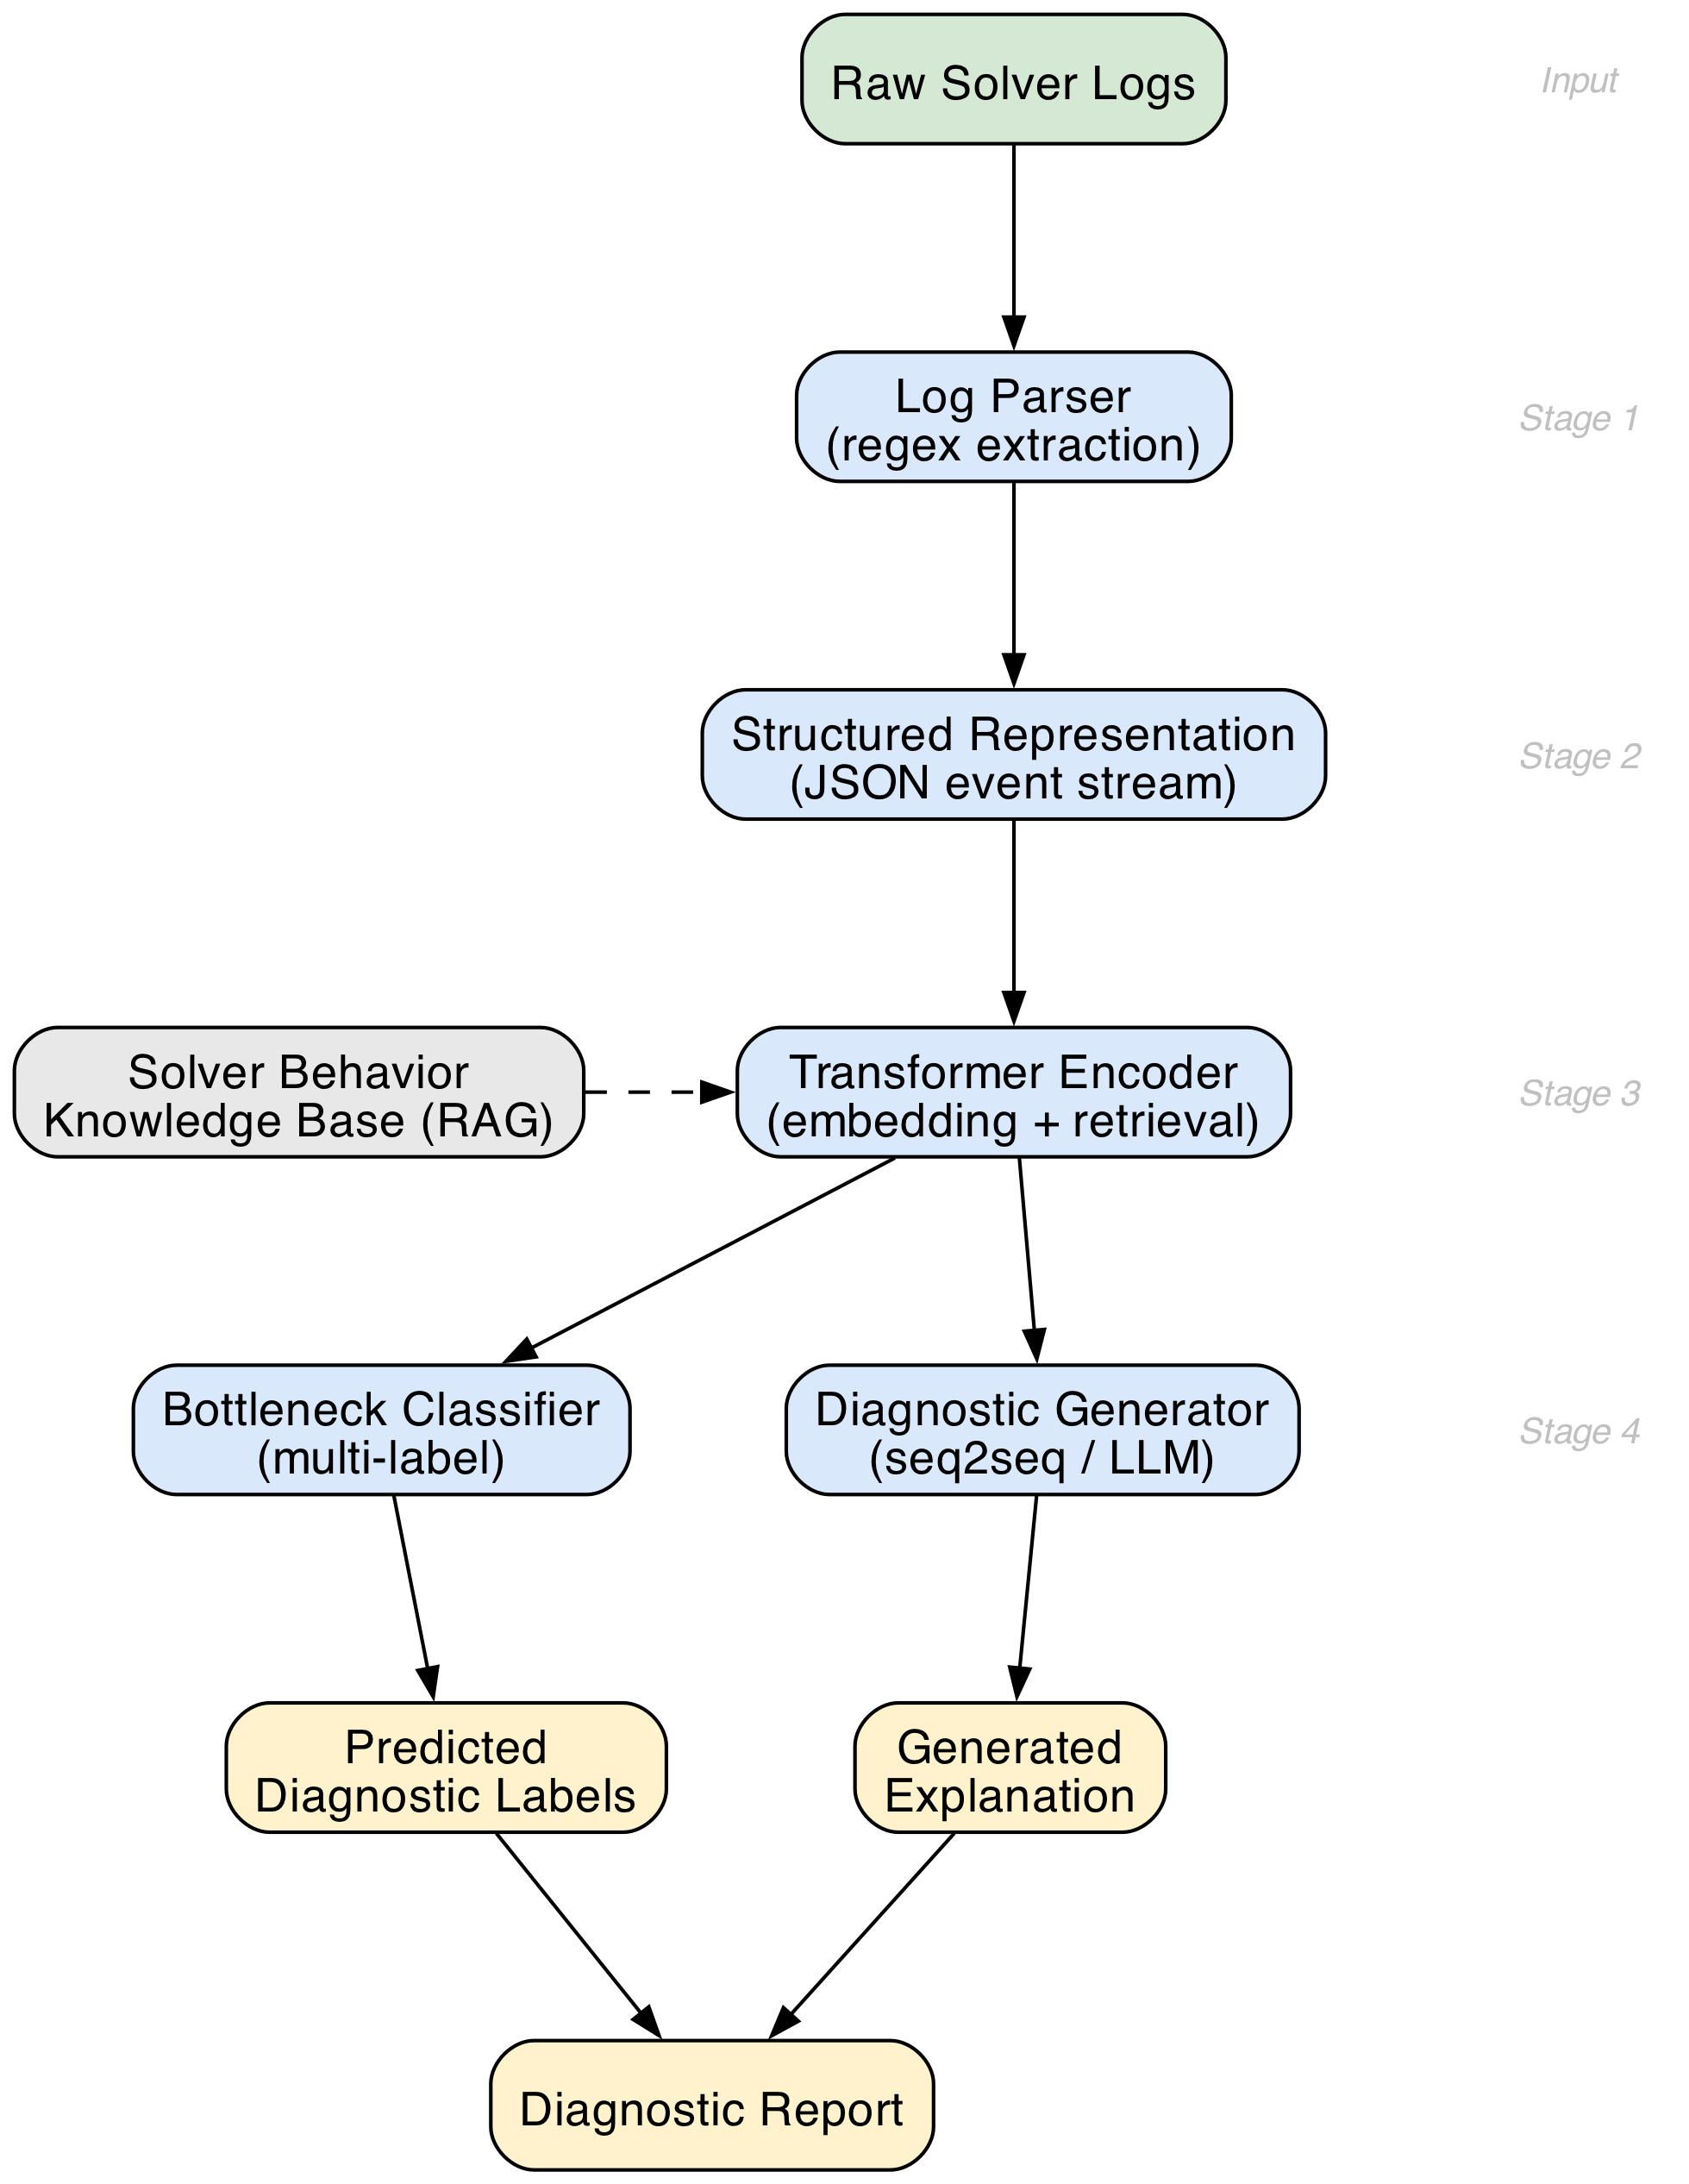
\includegraphics[width=0.70\textwidth]{architecture.png}
\caption{Optimization Log Copilot system architecture. Raw solver logs are parsed into structured JSON events, encoded via a transformer, and processed by: a multi-label bottleneck 
classifier and a seq2seq diagnostic generator. An RAG knowledge base augments the encoder with known solver behavior patterns.}
\label{fig:architecture}
\end{figure}

\begin{enumerate}
    \item Log Parsing: Raw solver log text is parsed into a structured event stream. A regex-based parser extracts key fields including model dimensions, presolve statistics, 
    root relaxation objective, node-by-node progress (incumbent, best bound, gap), cutting plane counts by type, heuristic solutions found, and termination status.
    \item Structured Representation: Parsed events are converted into a JSON-based structured format that captures the progression of the solve. Each log is represented as 
    a sequence of events with associated metrics, enabling downstream models to reason over solver progress more effectively than using raw text alone.
    \item Embedding and Retrieval: Structured log representations are embedded using a transformer encoder. 
    \item LLM Reasoning and Generation: The language model receives the structured log representation (and optionally retrieved examples) and produces a diagnostic report 
    containing a summary of solver behavior, predicted bottleneck labels, and recommended actions.
\end{enumerate}

\subsection{Dataset Construction}
\label{sec:dataset}

The dataset consists of approximately 200 solver logs collected from two sources:
\begin{itemize}
    \item MIPLIB 2017 benchmarks: Standard benchmark instances from the Mixed Integer Programming Library (\url{https://miplib.zib.de/}), 
    representing a diverse set academic MIP problems.
    \item Ramsey-type problems: A series of combinatorial models representing Ramsey problems (e.g., $R(4,4;15)$), which exhibit a 
    range of solver behaviors including symmetry, large search trees, infeasibility, and difficult relaxations.
\end{itemize}

Logs have been generated using the Rose solver. An automated benchmarking pipeline enables generation of additional logs as needed. The logs cover a 
range of solver behaviors, including optimal solutions, infeasible instances, various cutting plane and heuristic strategies, difficult root relaxations, varying 
optimality gap closures, a wide variety of node counts, and degenerate problems.

Each training example is constructed as a triple:
\begin{equation}
    (\text{log\_text}, \text{diagnostic\_labels}, \text{explanation})
\end{equation}
where log\_text is the cleaned solver log, 
diagnostic\_labels is a multi-hot vector of bottleneck categories, and 
explanation is a natural-language summary describing solver behavior and potential improvements. 
Initial labels are generated using heuristic rules derived from solver metrics (e.g., root gap $>$ 30\% $\rightarrow$ ``weak relaxation'', node count $>$ 100{,}000 $\rightarrow$ ``excessive branching'') 
and then refined through manual expert review.

\subsection{Bottleneck Classification Model}

The classification component is formulated as a multi-label classification problem. Given a solver log, the model predicts a probability for each bottleneck category. 
The label set includes:

\begin{table}[h]
\centering
\begin{tabular}{ll}
\toprule
\textbf{Label} & \textbf{Indicator} \\
\midrule
Weak root LP & Large initial optimality gap \\
Branching difficulty & High node count \\
Degeneracy & Slow LP pivots \\
Ineffective cuts & Many rounds, little bound improvement \\
Presolve weakness & Minimal variable/constraint reduction \\
\bottomrule
\end{tabular}
\label{tab:labels}
\end{table}

The classification model uses a transformer encoder to generate contextual representations of the log text. Since solver logs can be long, architectures designed for long sequences such 
as Longformer \cite{beltagy2020longformer} or Big Bird \cite{zaheer2020bigbird} are candidates.

\subsection{Generative Explanation Model}

To produce human-readable diagnostics, a sequence-to-sequence generative model (e.g., T5 or FLAN-T5) generates explanations conditioned on the solver log and predicted diagnostic labels. 

Following standard autoregressive sequence modeling used in transformer architectures (\cite{raffel2020t5}), the probability of the generated explanation is factorized into the product of conditional token probabilities:
\begin{equation}
    P(\text{explanation} \mid \text{log\_text}, \text{labels}) = \prod_{t=1}^{T} P(w_t \mid w_{<t}, \text{log\_text}, \text{labels})
\end{equation}
where $w_t$ denotes the $t$-th token of the generated explanation. The model is trained to produce concise summaries describing solver behavior and recommend potential improvements to model 
formulation or solver configuration.

\subsection{LLM Approach Comparison}

Three LLM-based approaches will be evaluated:
\begin{enumerate}
    \item Prompt Engineering: Directly feeding solver logs to a pre-trained LLM with domain-specific prompts. This is the simplest approach and requires no training data.
    \item Retrieval-Augmented Generation (RAG): Augmenting the LLM with a database of known solver behavior patterns and diagnostic examples. The system retrieves relevant examples based on log similarity before generating a response.
    \item Fine-Tuning: Training a smaller model on the labeled dataset of solver logs and expert annotations. This approach requires the most data but may produce the most consistent domain-specific outputs.
\end{enumerate}

Based on findings from the literature \cite{akhtar2025llmbasedeventloganalysis}, RAG is expected to offer the best balance of accuracy and practicality for this domain, given the relatively small dataset size and the need to reduce hallucination risk.

% ============================================================
\section{Experimental Plan}
\label{sec:experiments}

\textit{[This section will be completed in the final paper.]}

The experimental evaluation will assess the system using three performance metrics, each tied to a sub-hypothesis. Together, they provide a quantitative framework for determining whether the primary hypothesis holds.

\subsection{Metric 1: Macro-Averaged F1 Score for Bottleneck Detection (H1)}

The first metric evaluates the multi-label classification component. For each bottleneck category $k \in \{1, \ldots, K\}$, precision ($P_k$), recall ($R_k$), and F1 ($F_{1,k}$) are computed in the standard way:
\begin{equation}
    P_k = \frac{TP_k}{TP_k + FP_k}, \quad R_k = \frac{TP_k}{TP_k + FN_k}, \quad F_{1,k} = \frac{2 P_k R_k}{P_k + R_k}
\end{equation}
The macro-averaged F1 score is the unweighted mean across all $K=5$ bottleneck categories:
\begin{equation}
    F_1^{\text{macro}} = \frac{1}{K} \sum_{k=1}^{K} F_{1,k}
\end{equation}

The target threshold is $F_1^{\text{macro}} \geq 0.85$. This is grounded in results from Landauer et al.\ \cite{landauer2023deeplearningloganomaly}, who report F1 scores of 0.90--0.98 for deep LSTM-based log anomaly detectors and often exceeding 0.95 for transformer-based approaches. The lower threshold of 0.85 accounts for the smaller dataset size (approximately 200 logs vs.\ thousands in IT log benchmarks) and the specialized domain. The metric will be computed on a held-out test set (20\% of logs) using 5-fold cross-validation to account for dataset size. Both the rule-based baseline and each LLM approach (prompt engineering, RAG, fine-tuning) will be evaluated on the same folds.

\subsection{Metric 2: ROUGE-L Score for Diagnostic Summarization (H2)}

The second metric evaluates the quality of generated diagnostic summaries. ROUGE-L measures the longest common subsequence (LCS) between a generated summary $S$ and a reference summary $R$:
\begin{equation}
    P_{\text{lcs}} = \frac{|LCS(S, R)|}{|S|}, \quad R_{\text{lcs}} = \frac{|LCS(S, R)|}{|R|}, \quad \text{ROUGE-L} = \frac{(1 + \beta^2) P_{\text{lcs}} R_{\text{lcs}}}{\beta^2 P_{\text{lcs}} + R_{\text{lcs}}}
\end{equation}
with $\beta$ set to favor recall ($\beta = 1.2$), following standard practice. ROUGE-1 and ROUGE-2 (unigram and bigram overlap) will also be reported for completeness.

The target threshold is ROUGE-L $\geq 0.40$. Raffel et al.\ \cite{raffel2020t5} report ROUGE-L scores in the 0.35--0.45 range for T5 on abstractive summarization benchmarks. Because solver log summaries require domain-specific terminology (e.g., ``root LP relaxation,'' ``branching pseudocosts'') and precise numerical claims (e.g., ``gap closed from 40\% to 5\%''), achieving ROUGE-L $\geq 0.40$ would demonstrate that generated summaries capture the substantive content of expert-written references rather than producing superficially similar generic text. Reference summaries will be written by the author for each test log, describing the key solver behavior, identified bottlenecks, and performance characteristics.

\subsection{Metric 3: Expert Actionability Rate for Recommendations (H3)}

The third metric evaluates whether generated recommendations are practically useful. Each recommendation produced by the system will be presented to a domain expert (the author, with experience in optimization solver configuration) alongside the corresponding solver log. The expert assigns a binary label: \emph{actionable and correct} (the recommendation identifies a real issue and suggests a plausible intervention) or \emph{not actionable} (the recommendation is vague, incorrect, or irrelevant). The actionability rate is:
\begin{equation}
    A = \frac{\text{number of recommendations rated actionable}}{\text{total recommendations evaluated}}
\end{equation}

The target threshold is $A \geq 0.70$. This threshold is motivated by Akhtar et al.\ \cite{akhtar2025llmbasedeventloganalysis}, who find that LLM-based log analysis systems should supplement rather than replace human reasoning, and that hallucination risk makes perfect accuracy unrealistic. A 70\% actionability rate would demonstrate that the majority of generated recommendations provide genuine diagnostic value. To mitigate single-rater bias, a subset of recommendations will be evaluated independently by a second reviewer, and inter-rater agreement (Cohen's kappa) will be reported.

\subsection{Planned Experiments}

\begin{enumerate}
    \item Baseline comparison: Compare the rule-based heuristic baseline (implemented in the prototype notebook) against each LLM approach on all three metrics to quantify the improvement from learned models.
    \item Approach comparison: Evaluate prompt engineering, RAG, and fine-tuning on the same held-out test set to determine which strategy is most effective for solver log analysis. Results will be reported per-metric with 95\% confidence intervals.
    \item Sensitivity analysis: Assess how each metric varies with dataset size by evaluating on subsets of 50, 100, and 200 logs to determine whether the current dataset is sufficient or whether additional log collection is needed.
\end{enumerate}

\subsection{Planned Statistical Analysis}

For Metric 1, statistical significance between approaches will be assessed using a paired bootstrap test over the cross-validation folds. For Metric 2, significance will be assessed using a paired permutation test on per-log ROUGE-L scores. For Metric 3, confidence intervals on the actionability rate will be computed using the Wilson score interval, which is appropriate for proportions with moderate sample sizes. All comparisons will use a significance level of $\alpha = 0.05$.

% ============================================================
\section{Results}
\label{sec:results}

\textit{[This section will be completed in the final paper. Preliminary prototype results from rule-based log parsing and heuristic diagnostics are available in the accompanying Jupyter notebook.]}

% ============================================================
\section{Conclusion and Future Work}
\label{sec:conclusion}

\textit{[This section will be completed in the final paper.]}

This project explores the use of large language models to interpret optimization solver logs and provide automated diagnostics for mathematical optimization problems. By combining structured 
log parsing with LLM reasoning, the Optimization Log Copilot aims to assist both researchers and practitioners in understanding solver behavior and improving optimization performance.

Possible future directions include: application to logs from additional solvers such as Gurobi, HiGHS, and CPLEX; interactive solver debugging via a conversational interface; automated parameter tuning recommendations; and 
integration into solver frameworks.

% ============================================================
\begin{thebibliography}{99}

    \bibitem{akhtar2025llmbasedeventloganalysis}
    S.~Akhtar, S.~Khan, and S.~Parkinson, ``LLM-based event log analysis techniques: A survey,''
    \emph{arXiv preprint arXiv:2502.00677}, 2025.
    [Online]. Available: \url{https://arxiv.org/abs/2502.00677}

    \bibitem{landauer2023deeplearningloganomaly}
    M.~Landauer, S.~Onder, F.~Skopik, and M.~Wurzenberger, ``Deep learning for anomaly detection in log data: A survey,''
    \emph{Machine Learning with Applications}, vol.~12, p.~100470, 2023.
    [Online]. Available: \url{https://www.sciencedirect.com/science/article/pii/S2666827023000233}

    \bibitem{bengio2018mlforcombinatorial}
    Y.~Bengio, A.~Lodi, and A.~Prouvost, ``Machine learning for combinatorial optimization: A methodological tour d'horizon,''
    \emph{arXiv preprint arXiv:1811.06128}, 2018.
    [Online]. Available: \url{https://arxiv.org/abs/1811.06128}

    \bibitem{kotary2021endtoend}
    J.~Kotary, F.~Fioretto, P.~Van~Hentenryck, and B.~Wilder, ``End-to-end constrained optimization learning: A survey,''
    in \emph{Proceedings of the International Joint Conference on Artificial Intelligence (IJCAI)}, 2021.
    [Online]. Available: \url{https://arxiv.org/abs/2103.16378}

    \bibitem{yazdani2025evocut}
    M.~Yazdani, M.~Mostajabdaveh, S.~Aref, and Z.~Zhou, ``EvoCut: strengthening integer programs via evolution-guided language models,''
    \emph{arXiv preprint arXiv:2508.11850}, 2025.
    [Online]. Available: \url{https://arxiv.org/abs/2508.11850}

    \bibitem{beltagy2020longformer}
    I.~Beltagy, M.~E.~Peters, and A.~Cohan, ``Longformer: The long-document transformer,''
    \emph{arXiv preprint arXiv:2004.05150}, 2020.
    [Online]. Available: \url{https://arxiv.org/abs/2004.05150}
    
    \bibitem{zaheer2020bigbird}
    M.~Zaheer, G.~Guruganesh, A.~Dubey, J.~Ainslie, C.~Alberti, S.~Ontañón, P.~Pham, Q.~Wang, A.~Ravula, L.~Yang, and A.~Ahmed, ``Big Bird: Transformers for longer sequences,''
    \emph{arXiv preprint arXiv:2007.14062}, 2020.
    [Online]. Available: \url{https://arxiv.org/abs/2007.14062}

    \bibitem{raffel2020t5}
    C. Raffel, N. Shazeer, A. Roberts, K. Lee, S. Narang, M. Matena, Y. Zhou, W. Li, and P. J. Liu,
    ``Exploring the Limits of Transfer Learning with a Unified Text-to-Text Transformer,''
    \textit{Journal of Machine Learning Research}, vol. 21, no. 140, pp. 1--67, 2020.
\end{thebibliography}

\end{document}
